%!TEX root = practicum1.tex
Since \autoref{eq:1:lsChance} only holds when the points are general position we sampled them from a Gaussian distribution for both experiments, since the points are then guaranteed to be linearly independent \cite[Chapter~5]{prince2012computer}. In these experiments we have made the number of patterns dependent upon some parameter $\alpha$ according to: 
	\begin{equation}\label{eq:alpha}
		N = \alpha d.
	\end{equation}
We define $Q_{l.s.}$ as the fraction of data sets where the perceptron found a hyperplane to separate the two classes within the $d_{max}$ epochs.	

\subsection*{Experiment I}\label{ssec:experimentI}
For the first experiment we have sampled 500 50-dimensional from a standard normal distribution. The number of data points per data set is dependent upon \eqref{eq:alpha}, $d_{max}$ was set to 1000. The ratio $Q_{l.s.}$ for different values of $\alpha$ is plotted in \autoref{fig:experiment1:plot}.

\begin{figure}[H]
	\centering
	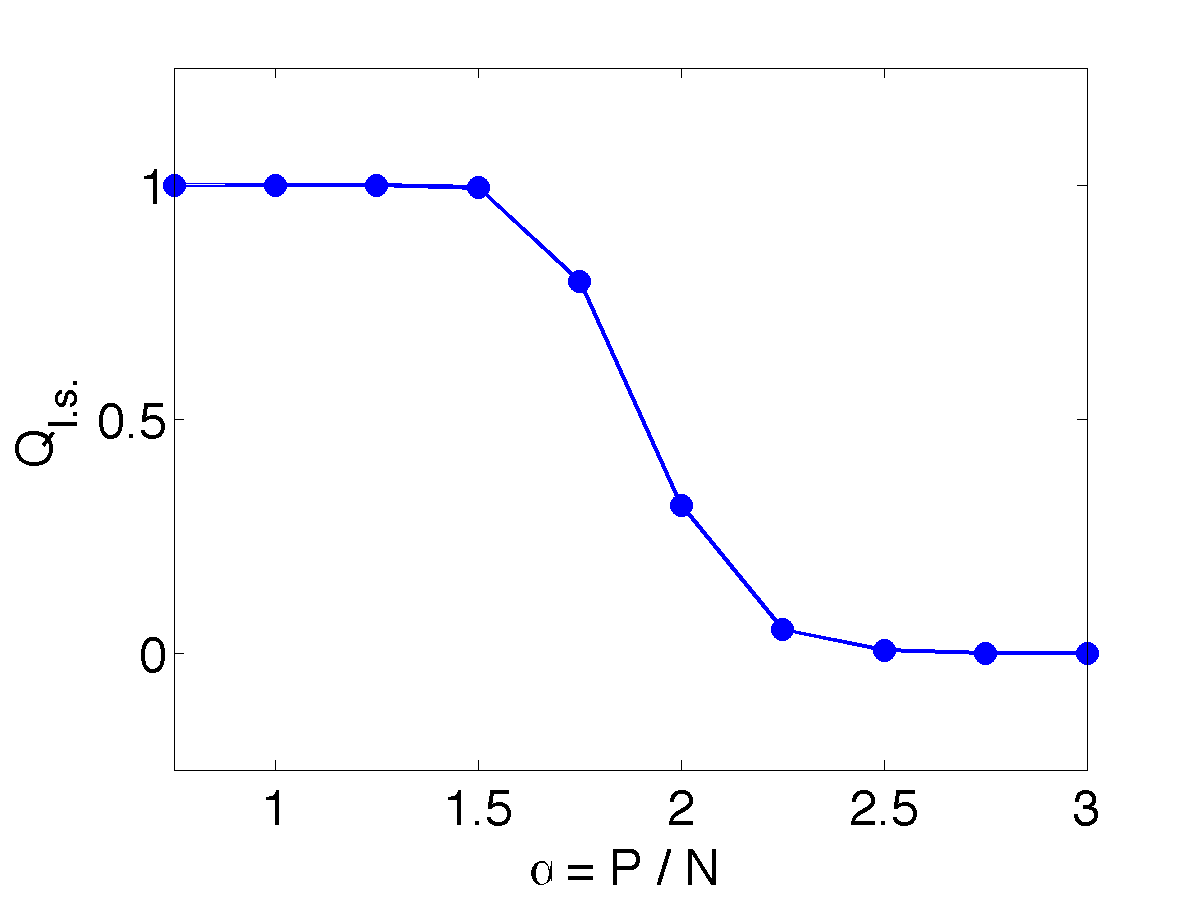
\includegraphics[width=\columnwidth]{./img/Aa_N50_nd500_nmax1000}
	\caption{The found relation between $\alpha$ and $Q_{l.s.}$, shown in blue, and the theoretical relation in red.}
	\label{fig:experiment1:plot}
\end{figure}

Using that $d = 50$  and substituting \eqref{eq:alpha} into the condition of the first case of \eqref{eq:1:lsChance} we find that $f(N,d)$ should be one for $\alpha \leq 1.02$. This fits with our results, which show that $Q_{l.s.}$ is one for all tested values of $\alpha$ that are smaller than or equal to 1.02. 

For $\alpha \in [1.5, 2.5]$ we find that the empirical $Q_{l.s.}$ is a bit lower than the theoretical value. The first of two possible causes is that the parameter $d_{max}$ was set too low. The perceptron convergence theorem states that the perceptron eventually converges, not necessarily after 500 steps. Another possible explanation is the fact that we are talking about chances, and that we just happened to get higher proportion of non-linearly separable datasets than theory predicts. 

For $\alpha \geq 2.5$ we find that the theoretical and empirical results coincide once again this is due to $f(N,d)$ approaching zero.

\subsection*{Experiment II}
% Observe the behavior of Ql.s. for different system sizes N as well. Does it approach a step function with increasing N? To this end, repeat the above experiments for, say, N = 50 and N = 100.

In this experiment we repeat the previous experiment I, with different sizes for $d$ in order to find if $Q_{l.s.}$ approaches the step function. The resulting plots of this experiment and the step function are shown in \vref{fig:2:experiment}. In the images in \cref{fig:2:experiment} we can see that when we the dimensionality increases the 

\begin{figure*}
	\centering
	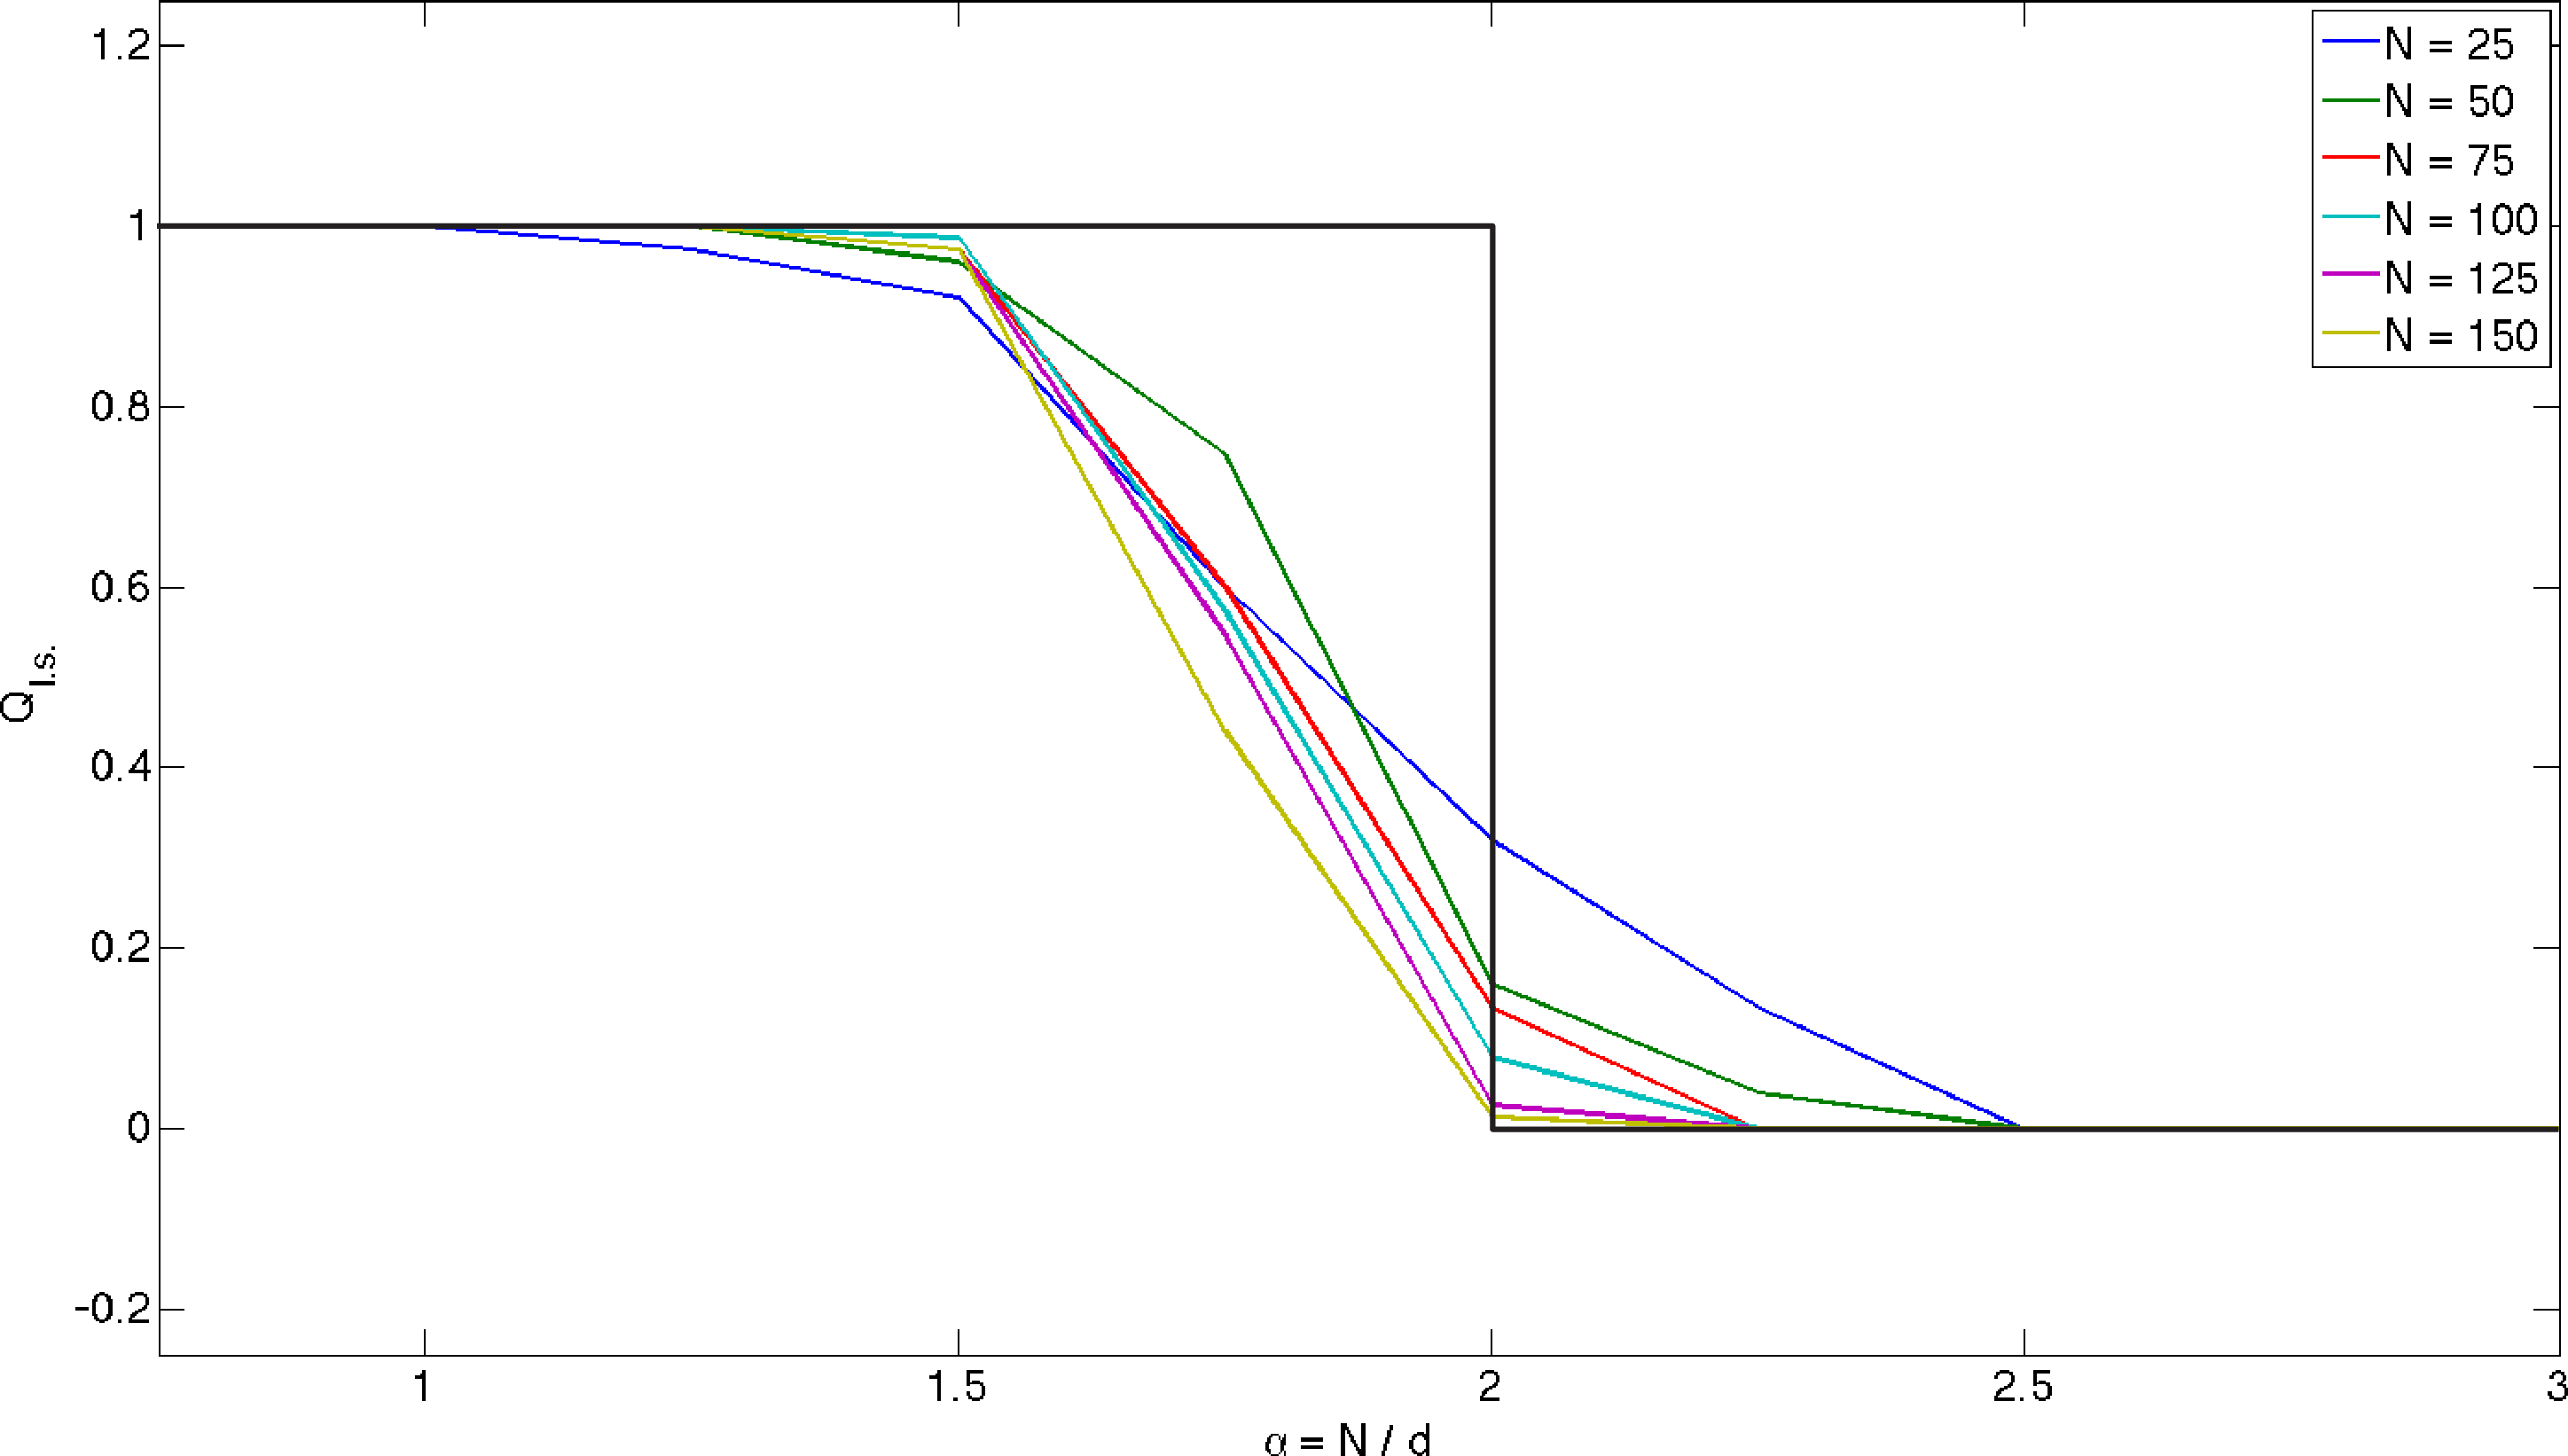
\includegraphics[width=\textwidth]{./img/assignmentb}
	\caption{Number of successful runs $Q_{l.s.}$ with different $d$}
	\label{fig:2:experiment}
\end{figure*}


\todo[inline]{Wat gaan we testen?}
\todo[inline]{Hoe gaan we het testen?}
\todo[inline]{Wat zijn onze onze resultaten}
\todo[inline]{In hoeverre kloppen de resultaten?}